% Provenance (never printed): cycle 4 SVT, "La planete Terre, l'environnement":
% glaciers and their landforms, the cryosphere, the glaciations told; see
% sources/book1/PROVENANCE.md. Book 1, grade 8, chapter 5.
% Vocabulary guard: owns glacier; ice sheet + ice shelf + iceberg (one
% definition); sea ice; permafrost; U-shaped valley + moraine (one
% definition); ice age. "Glacial period", "interglacial" and "glacial cycle"
% belong to Book 2 g12 past-climates: here "the ice ages and the warmer times
% between them", in prose. Albedo belongs to Book 2 g10: here "reflects".
% Buoyancy and water expanding as it freezes are physics: recalled in prose.
\chapter{IJs op Aarde}\label{ch:g8:ice-on-earth}

De twee foto's hieronder zijn vanaf dezelfde plek genomen, aan een lagune
in Alaska, met 26 jaar ertussen. In 1990 kwam er een brede ijstong door
het \omterm{def:g1:landscapes-around-us:landform}{dal} naar beneden, helemaal tot aan het water. In 2016 had het ijs zich
het \omterm{def:g1:landscapes-around-us:landform}{dal} in teruggetrokken en was het smaller geworden; bomen en kale rots
vulden de ruimte die het had achtergelaten. Satellietbeelden laten zien
dat het uiteinde van deze \omterm{def:g8:ice-on-earth:glacier}{gletsjer}, de Pedersengletsjer, tussen 1984 en 2021
ongeveer \qty{3.2}{km} is teruggeweken.
% ledger: commons:pedersen, uw:pedersen

\begin{omfigure}
\begin{minipage}[t]{0.49\linewidth}\centering
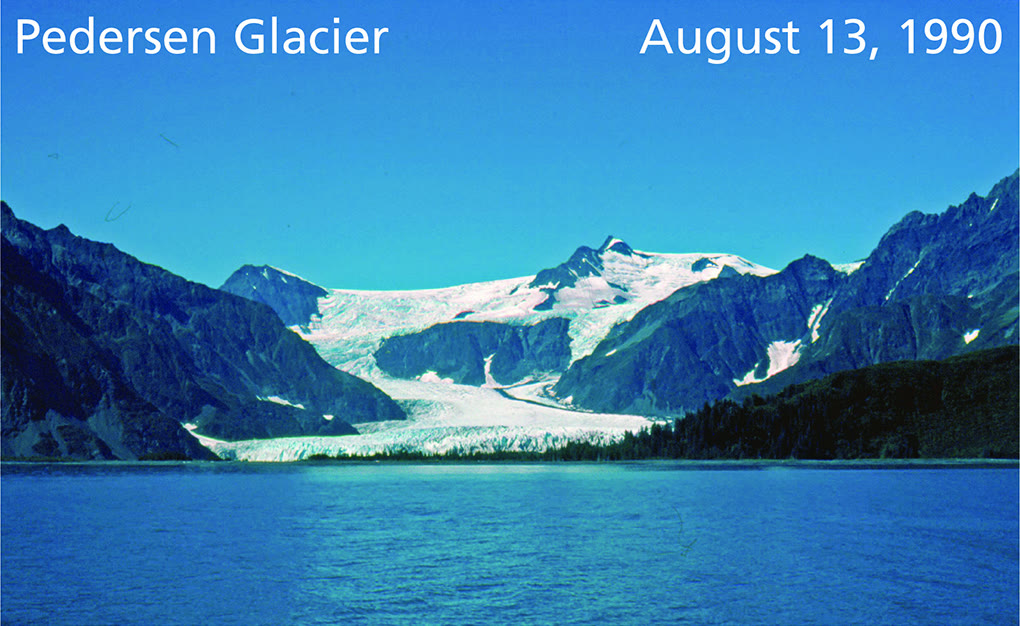
\includegraphics[width=\linewidth]{images/book1/g8-pedersen-1990.jpg}
\end{minipage}\hfill
\begin{minipage}[t]{0.49\linewidth}\centering
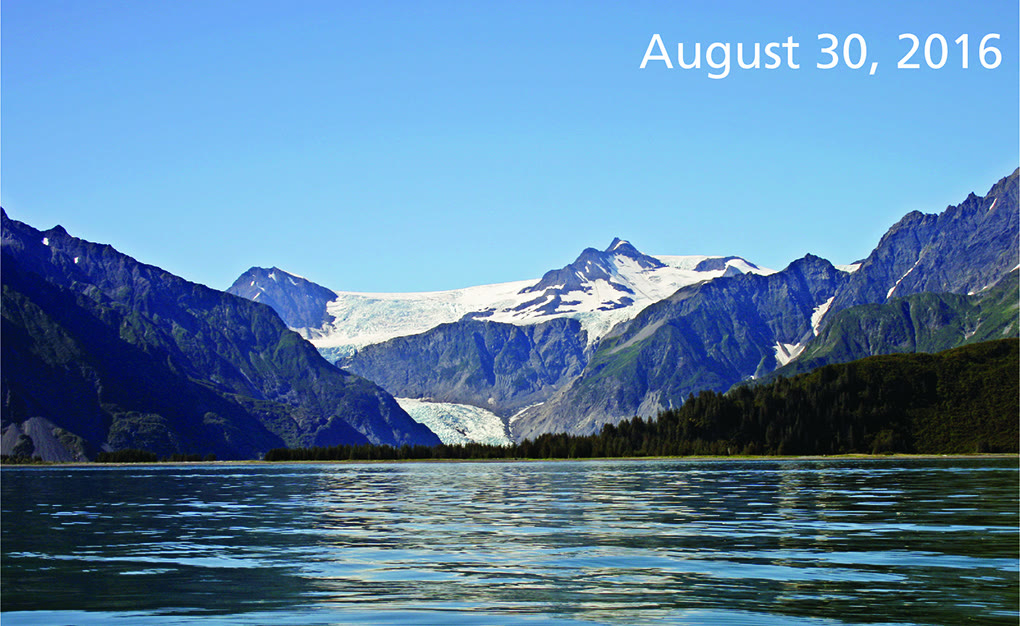
\includegraphics[width=\linewidth]{images/book1/g8-pedersen-2016.jpg}
\end{minipage}

\smallskip
{\small De Pedersengletsjer, Kenai Fjords National Park, Alaska, gezien
vanaf dezelfde plek op 13~augustus 1990 (links, foto van M.~Tetreau) en op
30~augustus 2016 (rechts, foto van D.~Kurtz). U.S. National Park
Service, publiek domein (via Wikimedia Commons).}
% ledger: commons:pedersen
\label{fig:g8:ice-on-earth:pedersen}
\end{omfigure}

IJs bedekt vandaag ongeveer een tiende van het land op Aarde. Het ligt in
bergdalen, in twee enorme kappen over Antarctica en Groenland, op de
poolzeeën en, verborgen, in de bevroren grond van het hoge noorden. Dit
hoofdstuk bekijkt ze een voor een, hoe ijs het land vormt, en de tijden
waarin ijs veel meer van de Aarde bedekte dan nu.
% ledger: nsidc:ice-cover

\begin{recall}
\omterm{def:g4:clouds-rain-snow:precipitation}{Sneeuw} is een vorm van \omterm{def:g4:clouds-rain-snow:precipitation}{neerslag}: ijskristallen die in een \omterm{def:g4:clouds-rain-snow:cloud}{wolk} groeien en
vallen zonder te smelten (\cref{ch:g4:clouds-rain-snow}). Stromend water
tast het land aan, voert de stukken mee en zet ze verderop af; een \omterm{def:g1:landscapes-around-us:water}{rivier}
snijdt een \omterm{def:g1:landscapes-around-us:landform}{dal} uit (\cref{ch:g5:water-shapes-the-land}). Als zeewater
bevriest, blijft het zout achter in het water rond het ijs
(\cref{ch:g8:the-oceans}). In de natuurkunde leer je dat water uitzet als
het bevriest, zodat ijs minder dicht is dan vloeibaar water, en dat een
voorwerp dat lichter is dan het water dat het verplaatst, blijft drijven.
\end{recall}

\section{Gletsjers}

Hoog in de \omterm{def:g1:landscapes-around-us:landform}{bergen} valt er in de winter meer \omterm{def:g4:clouds-rain-snow:precipitation}{sneeuw} dan er in de zomer
smelt. Jaar na jaar bedekt nieuwe \omterm{def:g4:clouds-rain-snow:precipitation}{sneeuw} de oude \omterm{def:g4:clouds-rain-snow:precipitation}{sneeuw} en drukt die
samen. De kristallen pakken samen, de lucht ertussen wordt eruit geperst,
en na ongeveer een jaar is de \omterm{def:g4:clouds-rain-snow:precipitation}{sneeuw} \emph{firn} geworden, een korrelig
materiaal tussen \omterm{def:g4:clouds-rain-snow:precipitation}{sneeuw} en ijs in. Steeds dieper begraven verandert de
firn in hard, massief ijs; bij de meeste \omterm{def:g8:ice-on-earth:glacier}{gletsjers} duurt dat meer dan
honderd jaar.
% ledger: nsidc:firn

\begin{definition}[Gletsjer]\label{def:g8:ice-on-earth:glacier}
Een \emph{gletsjer}\index{gletsjer} is een massa ijs, ontstaan uit \omterm{def:g4:clouds-rain-snow:precipitation}{sneeuw}
die zich vele jaren heeft opgehoopt, die onder haar eigen gewicht langzaam
over het land naar beneden beweegt.
\end{definition}
% ledger: nsidc:glacier-def

Een \omterm{def:g8:ice-on-earth:glacier}{gletsjer} heeft twee delen. In het bovenste deel, het
\emph{accumulatiegebied}, valt elk jaar meer \omterm{def:g4:clouds-rain-snow:precipitation}{sneeuw} dan er smelt: de
\omterm{def:g8:ice-on-earth:glacier}{gletsjer} wint ijs. In het onderste deel, het \emph{ablatiegebied}, smelt
elk jaar meer ijs dan er \omterm{def:g4:clouds-rain-snow:precipitation}{sneeuw} valt: de \omterm{def:g8:ice-on-earth:glacier}{gletsjer} verliest ijs. Het ijs dat
boven wordt gewonnen, blijft naar beneden stromen om het ijs te vervangen
dat onder verloren gaat. Als de twee in evenwicht zijn, blijft het
uiteinde van de \omterm{def:g8:ice-on-earth:glacier}{gletsjer}, zijn \emph{tong}, op dezelfde plaats.
% ledger: nsidc:glacier-zones

\begin{omfigure}
\begin{tikzpicture}[font=\footnotesize, >={Stealth[length=2mm]}, xscale=1.08]
  % bedrock
  \fill[black!13] (0,4.6) -- (2,3.9) -- (4,3.0) -- (6,2.0) -- (8,1.1)
    -- (10,0.45) -- (11,0.3) -- (13,0.15) -- (13,-0.5) -- (0,-0.5) -- cycle;
  % the ice body, two zones
  \begin{scope}
    \clip (0,5.5) -- (2,4.9) -- (4,4.0) -- (6,2.9) -- (8,1.8) -- (9.4,0.95)
      -- (10,0.45) -- (8,1.1) -- (6,2.0) -- (4,3.0) -- (2,3.9) -- (0,4.6) -- cycle;
    \fill[omIce] (0,-1) rectangle (5,6);
    \fill[omSea!85] (5,-1) rectangle (11,6);
  \end{scope}
  \draw[black!60] (0,5.5) -- (2,4.9) -- (4,4.0) -- (6,2.9) -- (8,1.8)
    -- (9.4,0.95) -- (10,0.45);
  \draw[black!70, line width=0.6pt] (0,4.6) -- (2,3.9) -- (4,3.0) -- (6,2.0)
    -- (8,1.1) -- (10,0.45) -- (11,0.3) -- (13,0.15);
  % snowline
  \draw[dashed, black!70] (5,2.5) -- (5,4.15);
  \node[anchor=south] at (5,4.15) {sneeuwval = smelten};
  % snowflakes and melting
  \foreach \x/\y in {0.5/6.1, 1.3/5.8, 2.1/5.5, 2.9/5.1, 3.7/4.8, 0.9/6.6, 1.7/6.3, 2.5/6.0, 3.3/5.6, 4.1/5.2}
    \node[omCold] at (\x,\y) {$\ast$};
  \foreach \x/\y in {6.4/2.8, 7.2/2.35, 8.0/1.9}
    \draw[omWarm, decorate, decoration={snake, amplitude=0.6mm, segment length=2mm}] (\x,\y) -- ++(0,0.6);
  % flow arrows inside the ice
  \draw[->, omDef, line width=0.9pt] (1.0,4.72) -- (2.2,4.30);
  \draw[->, omDef, line width=0.9pt] (3.0,3.95) -- (4.2,3.41);
  \draw[->, omDef, line width=0.9pt] (5.2,2.88) -- (6.4,2.28);
  \draw[->, omDef, line width=0.9pt] (7.2,1.84) -- (8.3,1.35);
  % moraine and meltwater
  \fill[omLithCongl] (10.15,0.42) .. controls (10.5,0.95) and (10.9,0.95) .. (11.2,0.29) -- cycle;
  \draw[omSea!60!black, line width=1.6pt] (10.05,0.38) .. controls (10.6,0.22) and (11.4,0.12) .. (12.9,0.08);
  % labels
  \node[align=center] at (1.9,7.15) {accumulatiegebied:\\ sneeuw hoopt zich op, de gletsjer wint ijs};
  \node[align=center] at (10.0,3.3) {ablatiegebied:\\ het ijs smelt, de gletsjer verliest ijs};
  \node[align=left, anchor=west, omDef] at (4.4,1.3) {het ijs stroomt\\ naar beneden};
  \draw[black!60] (10.0,0.5) -- (9.6,-0.1) node[below] {tong};
  \draw[black!60] (10.7,0.85) -- (11.3,1.4) node[above] {morene};
  \node[anchor=north east] at (12.9,0.0) {smeltwaterbeek};
  \node at (2.2,2.6) {vast gesteente};
\end{tikzpicture}

{\small Een dalgletsjer in lengtedoorsnede (een schets, niet op schaal).
Boven de stippellijn hoopt \omterm{def:g4:clouds-rain-snow:precipitation}{sneeuw} zich sneller op dan ze smelt; eronder
smelt het ijs sneller dan er \omterm{def:g4:clouds-rain-snow:precipitation}{sneeuw} valt. Het ijs stroomt van het ene deel
naar het andere.}
\label{fig:g8:ice-on-earth:long-section}
\end{omfigure}

Hoe kan vast ijs stromen? Onder het gewicht van het ijs erboven vervormt
het ijs diep in een \omterm{def:g8:ice-on-earth:glacier}{gletsjer} langzaam, zoals een dikke laag koude honing
uitvloeit. De \omterm{def:g8:ice-on-earth:glacier}{gletsjer} glijdt ook over de rots eronder, op een dun laagje
water of op natte modder. De onderkant van de \omterm{def:g8:ice-on-earth:glacier}{gletsjer}, die over de rots
schuurt, beweegt langzamer dan de bovenkant. De meeste \omterm{def:g8:ice-on-earth:glacier}{gletsjers} bewegen
langzaam en gelijkmatig; een paar gaan plotseling \emph{galopperen}. In
1986 schoof de Hubbardgletsjer in Alaska ongeveer \qty{10}{m} per dag
vooruit, en de snelste uitschieter die ooit is gemeten, de
Kutiahgletsjer in Pakistan in 1953, legde drie maanden lang gemiddeld
ongeveer \qty{112}{m} per dag af.
% ledger: nsidc:glacier-flow, nsidc:surges

Als een \omterm{def:g8:ice-on-earth:glacier}{gletsjer} onder meer ijs verliest dan hij boven wint, schuift zijn
tong het \omterm{def:g1:landscapes-around-us:landform}{dal} in omhoog: we zeggen dat de \omterm{def:g8:ice-on-earth:glacier}{gletsjer} \emph{zich terugtrekt}.
Een \omterm{def:g8:ice-on-earth:glacier}{gletsjer} die zich terugtrekt, stroomt nog steeds naar beneden, als een
lopende band; hij smelt alleen sneller dan hij stroomt. De Muirgletsjer in
Alaska vulde in 1941 zijn hele \omterm{def:g1:landscapes-around-us:landform}{dal} tot aan de \omterm{def:g2:water-on-earth:ocean}{zee}. In 2004 was zijn tong
\qty{12}{km} teruggeweken, en was het ijsoppervlak meer dan \qty{800}{m}
gezakt.
% ledger: nsidc:glacier-flow, nsidc:muir

\section{Hoe ijs een dal vormt}

Een \omterm{def:g8:ice-on-earth:glacier}{gletsjer} is een krachtig werktuig van \omterm{def:g5:water-shapes-the-land:erosion}{erosie}. Zijn ijs vriest vast aan
blokken los \omterm{def:g3:stones-pebbles-sand:rock}{gesteente} en rukt ze los; de stenen die in zijn onderkant zijn
vastgevroren, schuren de rots eronder als schuurpapier. De \omterm{def:g8:ice-on-earth:glacier}{gletsjer} voert
al dit \omterm{def:g3:stones-pebbles-sand:rock}{gesteente}, van fijn stof tot enorme rotsblokken, als een lopende
band het \omterm{def:g1:landscapes-around-us:landform}{dal} af, en laat het vallen waar het ijs smelt.
% ledger: nps:u-valley

\begin{omfigure}
\begin{tikzpicture}[font=\footnotesize, >={Stealth[length=2mm]}]
  % V-shaped valley
  \fill[black!13] (0,3) -- (2.1,0.35) -- (2.5,0.35) -- (4.6,3) -- (4.6,-0.4) -- (0,-0.4) -- cycle;
  \draw[black!70, line width=0.6pt] (0,3) -- (2.1,0.35) -- (2.5,0.35) -- (4.6,3);
  \fill[omSea] (2.1,0.35) -- (2.5,0.35) -- (2.42,0.2) -- (2.18,0.2) -- cycle;
  \node[align=center] at (2.3,-0.85) {een rivier snijdt een smal\\ V-dal uit};
  % arrow
  \draw[->, line width=1pt] (5.0,1.5) -- (6.2,1.5) node[midway, above, align=center] {een gletsjer\\ vult het};
  % U-shaped valley
  \begin{scope}[xshift=6.6cm]
    \fill[black!13] (0,3) .. controls (0.6,1.0) and (0.9,0.25) .. (1.6,0.2)
      -- (3.0,0.2) .. controls (3.7,0.25) and (4.0,1.0) .. (4.6,3) -- (4.6,-0.4) -- (0,-0.4) -- cycle;
    \draw[black!70, line width=0.6pt] (0,3) .. controls (0.6,1.0) and (0.9,0.25) .. (1.6,0.2)
      -- (3.0,0.2) .. controls (3.7,0.25) and (4.0,1.0) .. (4.6,3);
    \draw[dashed, black!40] (0,3) -- (2.1,0.35) -- (2.5,0.35) -- (4.6,3);
    \draw[omCold, line width=0.9pt] (0.37,2.2) -- (4.23,2.2);
    \node[omCold, anchor=south, font=\scriptsize] at (2.3,2.2) {vroeger ijsoppervlak};
    \fill[omLithCongl] (0.75,0.95) .. controls (0.95,1.2) and (1.1,1.1) .. (1.2,0.6) -- cycle;
    \fill[omLithCongl] (3.85,0.95) .. controls (3.65,1.2) and (3.5,1.1) .. (3.4,0.6) -- cycle;
    \node[align=center] at (2.3,-0.85) {als het ijs weg is: een breed\\ U-dal met steile wanden};
    \draw[black!60] (3.65,0.95) -- (4.85,0.6) node[right, align=left] {zij-\\ morene};
    \node[font=\scriptsize, black!55, align=center] at (2.3,1.6) {(oude V gestippeld)};
  \end{scope}
\end{tikzpicture}

{\small Hetzelfde bergdal in dwarsdoorsnede, voor en na een \omterm{def:g8:ice-on-earth:glacier}{gletsjer} (een
schets). Het ijs schuurt het smalle rivierdal uit tot een brede trog met
een vlakke bodem en steile wanden, en laat langs zijn randen ruggen van
puin achter.}
\label{fig:g8:ice-on-earth:v-and-u}
\end{omfigure}

\begin{definition}[U-dal en morene]\label{def:g8:ice-on-earth:glacial-landforms}
Een \emph{U-dal}\index{U-dal} is een \omterm{def:g1:landscapes-around-us:landform}{dal} met een brede, vlakke bodem en
steile wanden, uitgeslepen door een \omterm{def:g8:ice-on-earth:glacier}{gletsjer} die een smal V-vormig
rivierdal heeft verbreed en verdiept. Een \emph{morene}\index{morene} is
een rug van puin, van stof tot rotsblokken, die een \omterm{def:g8:ice-on-earth:glacier}{gletsjer} heeft
achtergelaten: een \emph{zijmorene} langs zijn zijkant, een
\emph{eindmorene} aan zijn uiteinde.
\end{definition}
% ledger: usgs:erratic, nps:u-valley, nps:moraines

\omterm{def:g8:ice-on-earth:glacial-landforms}{Morenen} zijn nuttige aanwijzingen. Een \omterm{def:g8:ice-on-earth:glacial-landforms}{eindmorene} ver beneden in een \omterm{def:g1:landscapes-around-us:landform}{dal},
zonder ijs in de buurt, laat zien hoe ver de \omterm{def:g8:ice-on-earth:glacier}{gletsjer} ooit reikte; een
\omterm{def:g8:ice-on-earth:glacial-landforms}{zijmorene} hoog op een dalwand laat zien hoe dik het ijs ooit was. Een groot
rotsblok dat alleen op een akker ligt, van een \omterm{def:g3:stones-pebbles-sand:rock}{gesteente} dat nergens in de
buurt voorkomt, is nog een aanwijzing: het is een \emph{zwerfsteen}, een
steen die door een \omterm{def:g8:ice-on-earth:glacier}{gletsjer} ver van zijn herkomst is meegevoerd en is
achtergebleven toen het ijs smolt. Zwerfstenen variëren van \omterm{def:g3:stones-pebbles-sand:pebble}{kiezels} tot
blokken die groter zijn dan een huis.
% ledger: nps:moraines, usgs:erratic

\begin{inthefield}[Een door ijs gevormd dal lezen]
Kijk tijdens een wandeling in de \omterm{def:g1:landscapes-around-us:landform}{bergen}, of op een foto van een bergdal,
naar de vorm van het \omterm{def:g1:landscapes-around-us:landform}{dal} in dwarsdoorsnede: een smalle V, of een brede U
met steile wanden? Zoek op de dalbodem naar lange ruggen van door elkaar
liggende stenen en aarde die langs de zijkanten of dwars door het \omterm{def:g1:landscapes-around-us:landform}{dal}
lopen: dat kunnen \omterm{def:g8:ice-on-earth:glacial-landforms}{morenen} zijn. Zoek naar grote rotsblokken die niet bij
het \omterm{def:g3:stones-pebbles-sand:rock}{gesteente} eromheen passen, en naar gladde rotsoppervlakken met lange
evenwijdige krassen. Blijf op de paden, blijf weg van de randen van steile
hellingen en van het ijs zelf, en teken wat je ziet in je schrift.
\end{inthefield}

\section{IJskappen, ijsplaten en ijsbergen}

De grootste ijsmassa's op Aarde liggen niet in bergdalen: ze bedekken
hele landen. De Antarctische \omterm{def:g8:ice-on-earth:ice-sheet}{ijskap} strekt zich uit over bijna
\num{14}~miljoen~\unit{km^2} en is op de dikste plek bijna \qty{4.9}{km}
dik. De Groenlandse \omterm{def:g8:ice-on-earth:ice-sheet}{ijskap} bedekt ongeveer \num{1.7}~miljoen~\unit{km^2},
vier vijfde van het eiland, en is meer dan \qty{3}{km} dik. Samen bevatten
ze meer dan 99~\% van het ijs op het land, en meer dan twee derde van al
het zoete water op Aarde.
% ledger: nsidc:ice-sheets

\begin{definition}[IJskap, ijsplaat en ijsberg]\label{def:g8:ice-on-earth:ice-sheet}
Een \emph{ijskap}\index{ijskap} is een massa ijs die meer dan
\qty{50000}{km^2} land bedekt, als een enorme koepel die zich naar alle
kanten uitspreidt. Waar ijs dat van het land af stroomt de \omterm{def:g2:water-on-earth:ocean}{zee} bereikt en
erop blijft drijven, nog vast aan het ijs erachter, vormt het een
\emph{ijsplaat}\index{ijsplaat}. Een \emph{ijsberg}\index{ijsberg} is een
groot blok ijs, meer dan \qty{5}{m} breed, dat van een \omterm{def:g8:ice-on-earth:glacier}{gletsjer} of een
ijsplaat is afgebroken en in \omterm{def:g2:water-on-earth:ocean}{zee} drijft.
\end{definition}
% ledger: nsidc:ice-sheets, nsidc:ice-shelves, nsidc:iceberg

\begin{omfigure}
\begin{minipage}[c]{0.5\linewidth}\centering
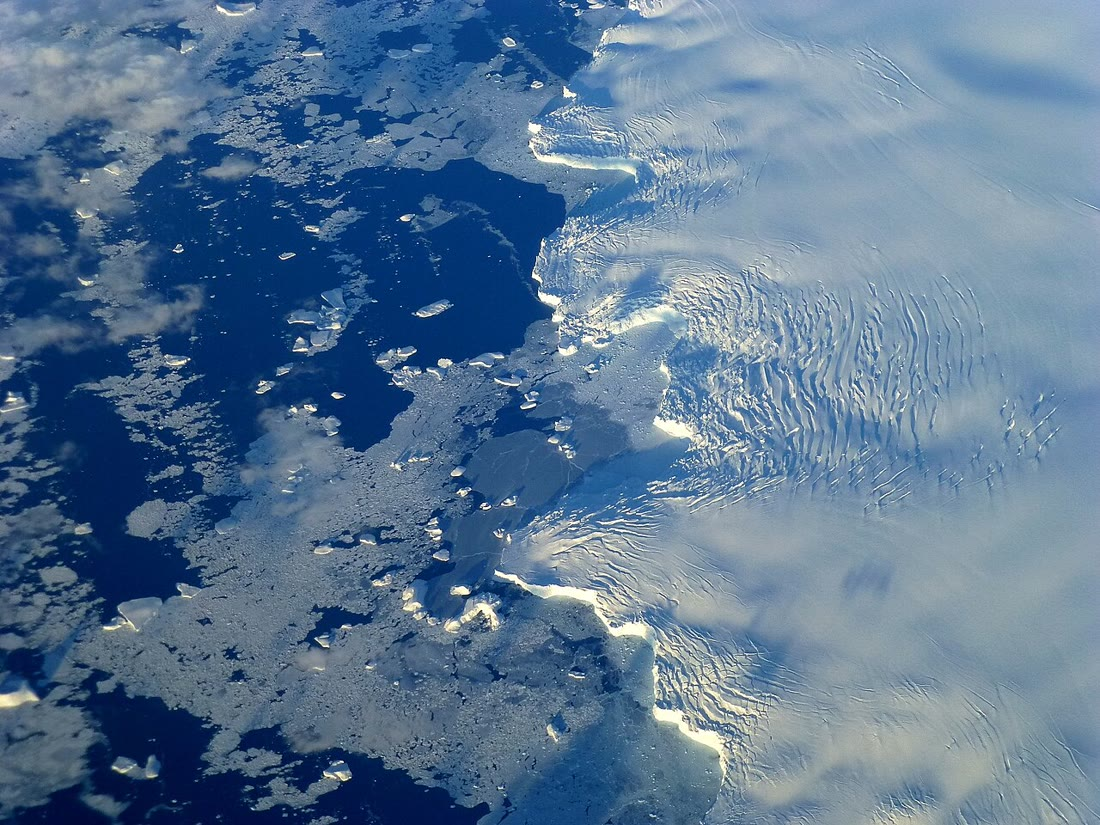
\includegraphics[width=\linewidth]{images/book1/g8-ice-shelf-edge.jpg}
\end{minipage}\hfill
\begin{minipage}[c]{0.46\linewidth}\raggedright
{\small De rand van een \omterm{def:g8:ice-on-earth:ice-sheet}{ijsplaat} bij Adelaide Island, voor het
Antarctisch Schiereiland, gezien vanuit een vliegtuig op 28~oktober 2012.
Het dikke, gerimpelde witte ijs rechts is de \omterm{def:g8:ice-on-earth:ice-sheet}{ijsplaat}; links drijven
gebroken stukken dunner \omterm{def:g8:ice-on-earth:sea-ice}{zee-ijs} op het donkere water. NASA, Operation
IceBridge (publiek domein, via Wikimedia Commons).}
\end{minipage}
% ledger: commons:ice-shelf
\label{fig:g8:ice-on-earth:ice-shelf}
\end{omfigure}

Het water dat in de \omterm{def:g8:ice-on-earth:ice-sheet}{ijskappen} vastzit, kwam uit de \omterm{def:g2:water-on-earth:ocean}{oceaan}: het verdampte,
viel als \omterm{def:g4:clouds-rain-snow:precipitation}{sneeuw} en hoopte zich op het land op. Als al het ijs van
Groenland smolt, zou de \omterm{def:g2:water-on-earth:ocean}{zee} ongeveer \qty{7.4}{m} stijgen; als al het ijs
van Antarctica smolt, ongeveer \qty{58}{m}. Alle berggletsjers van de
wereld, meer dan \num{200000}, zouden er minder dan een halve meter aan
toevoegen.
% ledger: nsidc:ice-sheets, nsidc:ice-cover

\begin{omfigure}
\begin{tikzpicture}
\begin{axis}[omrecord, xbar, width=10.5cm, height=3.6cm, xmin=0, xmax=68,
  bar width=9pt, ytick=data, symbolic y coords={gletsjers,Groenland,Antarctica},
  yticklabels={alle berggletsjers, Groenlandse ijskap, Antarctische ijskap},
  xlabel={stijging van de zee als alles smolt (m)}, enlarge y limits=0.3,
  nodes near coords, nodes near coords style={font=\footnotesize, anchor=west, fill=white, inner sep=1.5pt},
  ymajorgrids=false]
  \addplot[fill=omIce!80!black, draw=black!60] coordinates {(0.5,gletsjers) (7.4,Groenland) (58,Antarctica)};
\end{axis}
\end{tikzpicture}

{\small Hoeveel de \omterm{def:g2:water-on-earth:ocean}{zee} zou stijgen als elk soort landijs volledig smolt
(waarden van het National Snow and Ice Data Center; de waarde van de
\omterm{def:g8:ice-on-earth:glacier}{gletsjers} is een bovengrens, ``net iets minder dan een halve meter'').}
% ledger: nsidc:ice-sheets, nsidc:ice-cover
\label{fig:g8:ice-on-earth:sea-level-bars}
\end{omfigure}

Drijvend ijs is iets anders. Een \omterm{def:g8:ice-on-earth:ice-sheet}{ijsplaat} of een \omterm{def:g8:ice-on-earth:ice-sheet}{ijsberg} drijft al op de
\omterm{def:g2:water-on-earth:ocean}{zee}: hij heeft zijn eigen gewicht aan water al verplaatst. Als hij
uiteenvalt of smelt, stijgt de \omterm{def:g2:water-on-earth:ocean}{zee} niet. Maar een \omterm{def:g8:ice-on-earth:ice-sheet}{ijsplaat} houdt de
\omterm{def:g8:ice-on-earth:glacier}{gletsjers} erachter tegen, als een kurk in een fles; toen de \omterm{def:g8:ice-on-earth:ice-sheet}{ijsplaat}
Larsen~B op Antarctica in 2002 uiteenviel, gingen de \omterm{def:g8:ice-on-earth:glacier}{gletsjers} erachter
sneller stromen, sommige tot acht keer hun vroegere snelheid, en voerden
ze meer landijs naar de \omterm{def:g2:water-on-earth:ocean}{zee}.
% ledger: nsidc:ice-shelves

\begin{inthelab}[Drijvend ijs en ijs op het land]
Leg binnen in elk van twee doorzichtige glazen een steentje dat boven het
water uitsteekt als je ze vult. Laat in het eerste glas een paar ijsblokjes
op het water drijven. Leg in het tweede glas evenveel ijsblokjes op het
steentje, boven het water. Vul beide glazen tot dezelfde hoogte met water
en markeer die met een viltstift. Wacht tot al het ijs gesmolten is en
vergelijk dan de waterstanden met de streepjes. Welk glas gedraagt zich
als de \omterm{def:g2:water-on-earth:ocean}{zee} wanneer een \omterm{def:g8:ice-on-earth:ice-sheet}{ijsberg} smelt, en welk als de \omterm{def:g2:water-on-earth:ocean}{zee} wanneer een \omterm{def:g8:ice-on-earth:ice-sheet}{ijskap}
smelt?
\end{inthelab}

\section{Zee-ijs}

\omterm{def:g8:ice-on-earth:sea-ice}{Zee-ijs} is weer iets anders: het is de \omterm{def:g2:water-on-earth:ocean}{zee} zelf, bevroren. Elke winter
bevriest het oppervlak van de poolzeeën over een enorm gebied; elke zomer
smelt een groot deel van dit ijs weer. In het Noordpoolgebied is het ijs
het kleinst aan het eind van de zomer, in september, en het grootst aan
het eind van de winter, in maart. Satellieten meten sinds het eind van de
jaren 1970 elke dag zijn \emph{uitgestrektheid}: de oppervlakte \omterm{def:g2:water-on-earth:ocean}{zee} waar
minstens 15~\% van het oppervlak met ijs bedekt is.
% ledger: nsidc:sea-ice-def

\begin{definition}[Zee-ijs]\label{def:g8:ice-on-earth:sea-ice}
\emph{Zee-ijs}\index{zee-ijs} is bevroren zeewater: het ontstaat, groeit en
smelt in de \omterm{def:g2:water-on-earth:ocean}{oceaan} zelf. Het verschilt van \omterm{def:g8:ice-on-earth:ice-sheet}{ijsbergen} en \omterm{def:g8:ice-on-earth:ice-sheet}{ijsplaten}, die op
de \omterm{def:g2:water-on-earth:ocean}{zee} drijven maar zijn ontstaan uit \omterm{def:g4:clouds-rain-snow:precipitation}{sneeuw} die op het land is gevallen.
\end{definition}
% ledger: nsidc:sea-ice-def

\omterm{def:g8:ice-on-earth:sea-ice}{Zee-ijs} is van belang tot ver buiten de \omterm{def:g3:continents-and-oceans:poles}{polen}. Open zeewater is donker: het
weerkaatst maar ongeveer 6~\% van het zonlicht dat het bereikt en
absorbeert de rest. \omterm{def:g8:ice-on-earth:sea-ice}{Zee-ijs} weerkaatst 50 tot 70~\%, en \omterm{def:g8:ice-on-earth:sea-ice}{zee-ijs} met
\omterm{def:g4:clouds-rain-snow:precipitation}{sneeuw} erop tot 90~\%. Als het ijs smelt, absorbeert het donkere water
eronder meer van de energie van de Zon en warmt het op, waardoor er meer
ijs smelt.
% ledger: nsidc:sea-ice-reflect

\begin{omfigure}
\begin{tikzpicture}
\begin{axis}[omrecord, width=13cm, height=5.4cm, xmin=1977, xmax=2027,
  ymin=3, ymax=8.2, xtick={1980,1990,...,2020},
  x tick label style={/pgf/number format/1000 sep={}},
  xlabel={jaar}, ylabel={uitgestrektheid (miljoen km$^2$)},
  legend style={at={(0.98,0.97)}, anchor=north east, draw=none, fill=white}]
  \addplot[omCold, mark=*, mark size=1.3pt, line width=0.6pt]
    table[x=year, y=extent_Mkm2] {figdata/out/grade-8-sea_ice-extent.dat};
  \addlegendentry{gemiddelde uitgestrektheid in september}
  \addplot[omWarm, dashed, line width=1pt]
    table[x=year, y=extent_Mkm2] {figdata/out/grade-8-sea_ice-trend.dat};
  \addlegendentry{trendlijn}
  \node[font=\scriptsize, anchor=north] at (axis cs:2012,3.5) {2012};
\end{axis}
\end{tikzpicture}

{\small De uitgestrektheid van het Arctische \omterm{def:g8:ice-on-earth:sea-ice}{zee-ijs} in elke september,
1979--2025, en de rechte lijn die de punten het best volgt. Gegevens:
NSIDC Sea Ice Index, versie~4 (F.~Fetterer en anderen, 2025).}
% ledger: data:b1-nsidc-sea-ice (figdata/grade-8/sea_ice.py)
\label{fig:g8:ice-on-earth:sea-ice}
\end{omfigure}

De punten gaan van jaar tot jaar op en neer: het \omterm{def:g1:watching-the-weather:weather}{weer} van elke zomer telt
mee. Maar over de jaren heen \omterm{def:g1:landscapes-around-us:landform}{dalen} ze duidelijk. Om de verandering door de
schommelingen heen te zien, tekenen wetenschappers een \emph{trendlijn},
de rechte lijn die zo dicht mogelijk langs alle punten gaat.
% ledger: data:b1-nsidc-sea-ice (figdata/grade-8/sea_ice.py)

\begin{method}[Een trend in een grafiek lezen]
\begin{enumerate}
  \item Lees de assen: wat wordt er gemeten, in welke eenheid, over welke
        jaren.
  \item Kijk naar de punten: is er achter de schommelingen een algemene
        stijging, een algemene daling, of geen van beide?
  \item Lees de trendlijn af bij het eerste en bij het laatste jaar.
  \item Neem het verschil en deel door het aantal jaren (of decennia)
        ertussen: dat is de gemiddelde verandering per jaar (of per
        decennium).
  \item Lees niet te veel in één jaar: een enkel punt ver van de lijn is
        weer, de lijn is de trend.
\end{enumerate}
\end{method}

\begin{example}[Het septemberijs van het Noordpoolgebied]
Op de grafiek staat de trendlijn in 1979 op ongeveer
\num{7.6}~miljoen~\unit{km^2} en in 2025 op ongeveer
\num{4.1}~miljoen~\unit{km^2}. De verandering is $7.6 - 4.1 =
3.5$ miljoen~km$^2$ in $2025 - 1979 = 46$ jaar, dat is 4.6 decennia:
$3.5 \div 4.6 \approx 0.76$. Het septemberijs is met ongeveer
\num{0.76}~miljoen~\unit{km^2} per decennium gekrompen: in 46 jaar heeft
de trendlijn bijna de helft van haar waarde van 1979 verloren. Het
laagste punt, \num{3.57}~miljoen~\unit{km^2} in 2012, ligt ruim onder de
lijn: die zomer was uitzonderlijk.
\end{example}
% ledger: data:b1-nsidc-sea-ice (figdata/grade-8/sea_ice.py), nsidc:sea-ice-reflect

Metingen laten zien dat het zomerse \omterm{def:g8:ice-on-earth:sea-ice}{zee-ijs} van het Noordpoolgebied sinds
de jaren 1980 zowel kleiner als dunner is geworden, terwijl het
Noordpoolgebied opwarmde. \Cref{ch:g9:climate-past-and-present} bekijkt
hoe het \omterm{def:g5:weather-and-climate:climate}{klimaat} van de Aarde verandert, en waarom.
% ledger: nsidc:sea-ice-reflect

\section{Permafrost}

In het hoge noorden dringt de kou diep in de grond door. Onder de toendra
van Noord-Amerika, Groenland en Noord-Azië blijven de bodem en het
\omterm{def:g3:stones-pebbles-sand:rock}{gesteente} het hele jaar door bevroren, en vaak zijn ze dat al duizenden
jaren. Alleen een dunne bovenlaag, de \emph{actieve laag}, ontdooit elke
zomer en bevriest elke winter opnieuw; er groeien planten in, en water dat
niet in de bevroren grond eronder kan wegzakken, blijft in plassen aan het
oppervlak staan.
% ledger: nsidc:permafrost

\begin{definition}[Permafrost]\label{def:g8:ice-on-earth:permafrost}
\emph{Permafrost}\index{permafrost} is grond, bodem of \omterm{def:g3:stones-pebbles-sand:rock}{gesteente}, die
minstens twee jaar achter elkaar op of onder \qty{0}{\degreeCelsius}
blijft.
\end{definition}
% ledger: nsidc:permafrost

\omterm{def:g8:ice-on-earth:permafrost}{Permafrost} ligt onder ongeveer \num{23}~miljoen~\unit{km^2}, een kwart van
het land van het \omterm{def:g3:continents-and-oceans:equator}{noordelijk halfrond}, en onder ongeveer 85~\% van Alaska.
Bevroren grond vol ijs is zo hard als rots; als het ijs erin smelt, wordt
de grond modder en zakt hij in. Wegen barsten, gebouwen verzakken en
pijpleidingen kunnen breken: waar ze \omterm{def:g8:ice-on-earth:permafrost}{permafrost} kruist, loopt de
Trans-Alaska-pijpleiding over \qty{676}{km} boven de grond. Ontdooiende
\omterm{def:g8:ice-on-earth:permafrost}{permafrost} laat ook de resten van planten die er duizenden jaren in
bevroren zaten, vergaan, en daarbij komen koolstofdioxide en methaan in de
lucht.
% ledger: nsidc:permafrost, nsidc:permafrost-thaw

\begin{omfigure}
\begin{minipage}[c]{0.5\linewidth}\centering
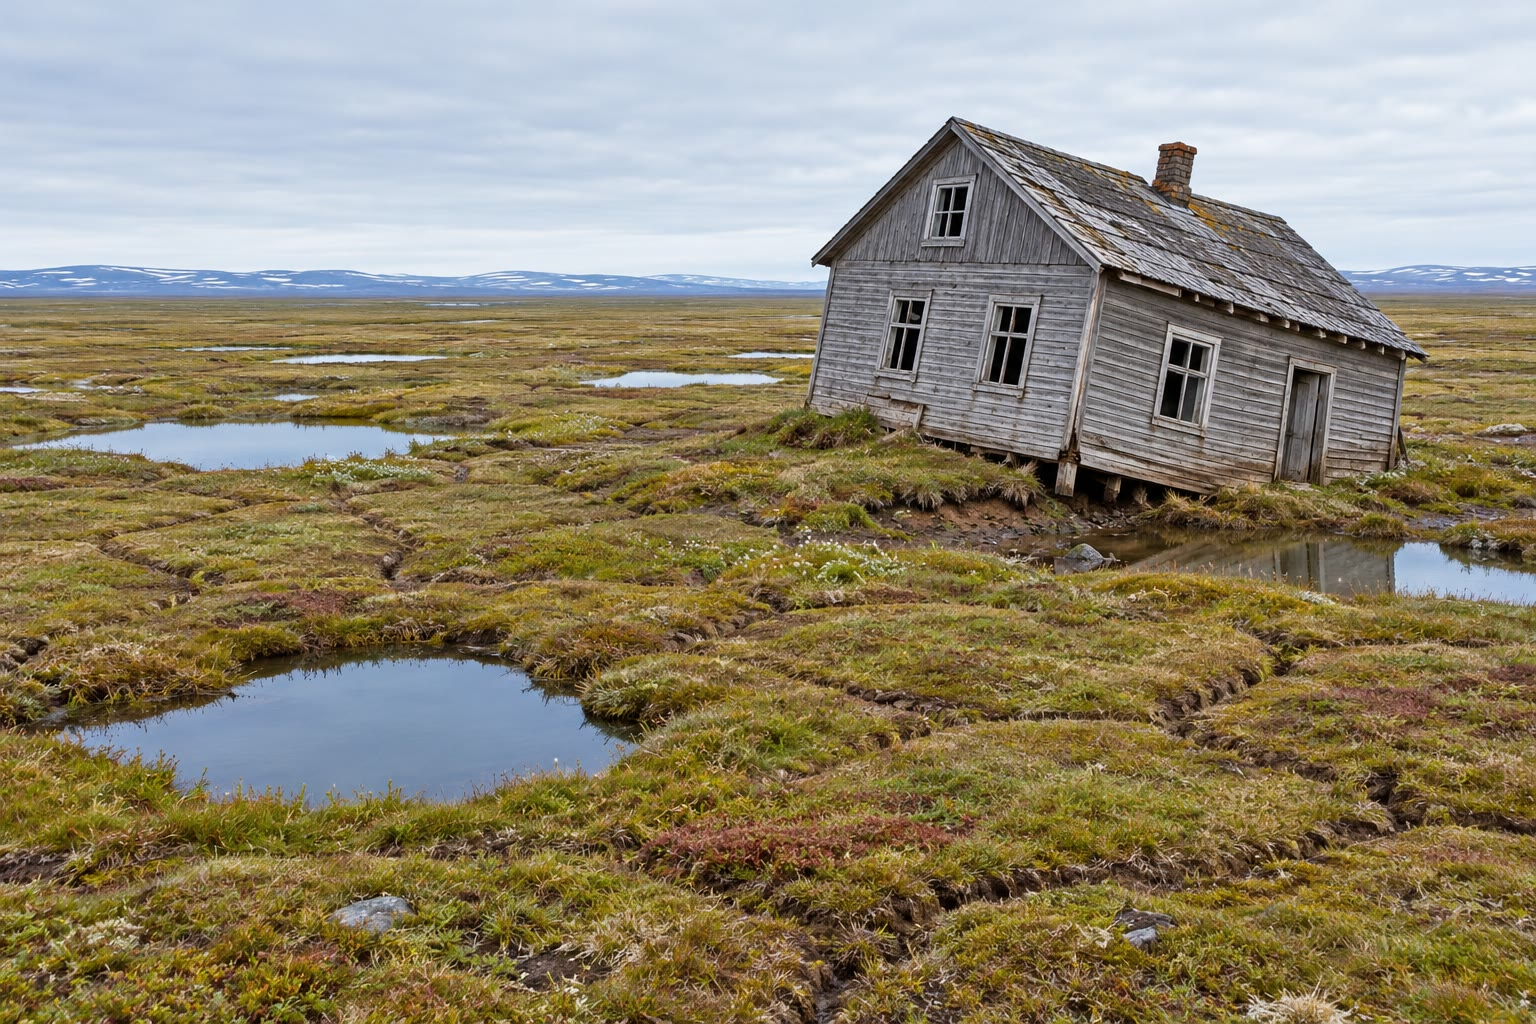
\includegraphics[width=\linewidth]{images/book1/ai/g8-permafrost-house.jpg}
\end{minipage}\hfill
\begin{minipage}[c]{0.46\linewidth}\centering
\begin{tikzpicture}[font=\footnotesize]
  \fill[omLithAlluv] (0,0) rectangle (3.2,-0.6);
  \fill[omIce!70!omLithShale] (0,-0.6) rectangle (3.2,-3.0);
  \foreach \x/\y in {0.4/-1.0, 1.5/-1.3, 2.6/-0.9, 0.9/-1.9, 2.1/-2.2, 0.5/-2.6, 2.8/-2.6}
    \fill[white] (\x,\y) ellipse (0.22 and 0.06);
  \fill[omLithShale!60] (0,-3.0) rectangle (3.2,-3.6);
  \draw[green!45!black, line width=1pt] (0,0) -- (3.2,0);
  \node[anchor=west, align=left] at (3.3,-0.3) {actieve laag:\\ ontdooit elke\\ zomer};
  \node[anchor=west, align=left] at (3.3,-1.8) {permafrost:\\ het hele jaar\\ bevroren, ijslenzen};
  \node[anchor=west, align=left] at (3.3,-3.3) {niet-bevroren\\ grond};
\end{tikzpicture}
\end{minipage}

\smallskip
{\small Links: een huis dat scheefzakt op ontdooiende \omterm{def:g8:ice-on-earth:permafrost}{permafrost} in de
toendra (door AI gegenereerde illustratie van een algemene scène).
Rechts: de grond onder de toendra (een schets, niet op schaal).}
\label{fig:g8:ice-on-earth:permafrost}
\end{omfigure}

\section{De ijstijden}

IJs heeft niet altijd hetzelfde deel van de Aarde bedekt. Ongeveer
\num{20000} jaar geleden bedekten \omterm{def:g8:ice-on-earth:ice-sheet}{ijskappen} een groot deel van
Noord-Amerika en van Noord-Europa, Scandinavië inbegrepen.
\omterm{def:g8:ice-on-earth:glacier}{Gletsjers} bedekten toen ongeveer een kwart van het land, tegen ongeveer een
tiende nu. Er zat zoveel water in dit ijs vast dat de \omterm{def:g2:water-on-earth:ocean}{zee} meer dan
\qty{120}{m} lager stond dan nu: delen van de huidige continentale platten
waren droog land. Vanaf ongeveer \num{15000} jaar geleden smolten de
\omterm{def:g8:ice-on-earth:ice-sheet}{ijskappen} terug en steeg de \omterm{def:g2:water-on-earth:ocean}{zee}; ze bereikte ongeveer \num{8000} jaar
geleden ruwweg haar huidige niveau.
% ledger: usgs:lgm, nsidc:ice-sheets, nsidc:ice-cover

\begin{definition}[IJstijd]\label{def:g8:ice-on-earth:ice-age}
Een \emph{ijstijd}\index{ijstijd} is een lange koude periode in de
geschiedenis van de Aarde waarin \omterm{def:g8:ice-on-earth:ice-sheet}{ijskappen} zich tot ver buiten de
poolgebieden uitbreiden en grote delen van de \omterm{def:g3:continents-and-oceans:continent}{continenten} bedekken. De
laatste ijstijd was ongeveer \num{20000} jaar geleden op zijn koudst en
eindigde ongeveer \num{12000} jaar geleden.
\end{definition}
% ledger: usgs:lgm, nps:u-valley

De sporen van de laatste \omterm{def:g8:ice-on-earth:ice-age}{ijstijd} zijn overal in de landen die hij bedekte:
\omterm{def:g8:ice-on-earth:glacial-landforms}{U-dalen} ver van elke huidige \omterm{def:g8:ice-on-earth:glacier}{gletsjer}, \omterm{def:g8:ice-on-earth:glacial-landforms}{eindmorenen} dwars over \omterm{def:g1:landscapes-around-us:landform}{vlakten},
zwerfstenen op akkers. En het was niet de enige. In de laatste paar
honderdduizend jaar hebben de \omterm{def:g8:ice-on-earth:ice-age}{ijstijden} en de warmere tijden ertussen
elkaar keer op keer opgevolgd; wij leven in een van de warme tijden.
\Cref{ch:g9:climate-past-and-present} vertelt hoe wetenschappers dit
lange verhaal lezen in het ijs van Antarctica zelf.
% ledger: nps:u-valley, nps:moraines, usgs:erratic

\section{Oefeningen}

\begin{exercise}[$\star$]\label{exo:g8:ice-on-earth:1}
Noem met de lengtedoorsnede van een \omterm{def:g8:ice-on-earth:glacier}{gletsjer} in dit hoofdstuk: (a) het
deel van de \omterm{def:g8:ice-on-earth:glacier}{gletsjer} waar hij ijs wint; (b) het deel waar hij ijs
verliest; (c) het uiteinde van de \omterm{def:g8:ice-on-earth:glacier}{gletsjer}; (d) de rug van puin aan zijn
uiteinde.
\end{exercise}

\begin{exercise}[$\star$]\label{exo:g8:ice-on-earth:2}
% ledger: nsidc:firn, nsidc:glacier-flow, nsidc:sea-ice-def
Waar of niet waar? Verbeter de onware zinnen. (a) Een \omterm{def:g8:ice-on-earth:glacier}{gletsjer} bestaat uit
bevroren zeewater. (b) \omterm{def:g4:clouds-rain-snow:precipitation}{Sneeuw} heeft ongeveer een jaar nodig om firn te
worden. (c) Als een \omterm{def:g8:ice-on-earth:glacier}{gletsjer} zich terugtrekt, stroomt zijn ijs omhoog.
(d) Het \omterm{def:g8:ice-on-earth:sea-ice}{zee-ijs} in het Noordpoolgebied is in september het kleinst.
\end{exercise}

\begin{exercise}[$\star$]\label{exo:g8:ice-on-earth:3}
% ledger: usgs:erratic, nsidc:permafrost
Geef het woord bij elke beschrijving: (a) een \omterm{def:g1:landscapes-around-us:landform}{dal} met een brede bodem en
steile wanden, uitgeslepen door ijs; (b) een rotsblok dat door een
\omterm{def:g8:ice-on-earth:glacier}{gletsjer} ver van zijn herkomst is meegevoerd; (c) een drijvende plaat ijs
die nog vastzit aan het ijs op het land; (d) grond die minstens twee jaar
achter elkaar bevroren blijft.
\end{exercise}

\begin{exercise}[$\star$]\label{exo:g8:ice-on-earth:4}
% ledger: nsidc:ice-sheets, nsidc:ice-cover
(a) Welke twee landen zijn vandaag door \omterm{def:g8:ice-on-earth:ice-sheet}{ijskappen} bedekt? (b) Welke van de
twee zou de \omterm{def:g2:water-on-earth:ocean}{zee} het meest laten stijgen als al zijn ijs smolt, en met
hoeveel? (c) Welk deel van het land op Aarde is vandaag door ijs bedekt?
\end{exercise}

\begin{exercise}[$\star\star$]\label{exo:g8:ice-on-earth:5}
% ledger: data:b1-nsidc-sea-ice (figdata/grade-8/sea_ice.py)
Gebruik de grafiek van het Arctische \omterm{def:g8:ice-on-earth:sea-ice}{zee-ijs} in september. (a) Lees de
uitgestrektheid af in 1979 en in 2012. (b) Met hoeveel miljoen~km$^2$ is
ze tussen deze twee jaren gekrompen? (c) Welk deel van de uitgestrektheid
van 1979 was in 2012 verdwenen? Rond af op een eenvoudige breuk.
(d) Waarom is het betrouwbaarder om de trendlijn te vergelijken dan twee
losse jaren?
\end{exercise}

\begin{exercise}[$\star\star$]\label{exo:g8:ice-on-earth:6}
% ledger: nsidc:muir, uw:pedersen
De tong van de Muirgletsjer is tussen 1941 en 2004 \qty{12}{km}
teruggeweken. (a) Hoeveel jaar is dat? (b) Hoeveel meter trok hij
gemiddeld per jaar terug? Rond af op tientallen meters. (c) De
Pedersengletsjer is tussen 1984 en 2021 \qty{3.2}{km} teruggeweken.
Hoeveel trok hij gemiddeld per jaar terug? (d) Welke \omterm{def:g8:ice-on-earth:glacier}{gletsjer} trok sneller
terug?
\end{exercise}

\begin{exercise}[$\star\star$]\label{exo:g8:ice-on-earth:7}
Leg in een paar zinnen en in de juiste volgorde uit hoe \omterm{def:g4:clouds-rain-snow:precipitation}{sneeuw} die hoog op
een \omterm{def:g1:landscapes-around-us:landform}{berg} valt, het ijs wordt van de tong van een \omterm{def:g8:ice-on-earth:glacier}{gletsjer}, ver beneden in
het \omterm{def:g1:landscapes-around-us:landform}{dal}. Gebruik de woorden \emph{firn}, \emph{accumulatiegebied},
\emph{stroomt} en \emph{ablatiegebied}.
\end{exercise}

\begin{exercise}[$\star\star$]\label{exo:g8:ice-on-earth:8}
% ledger: nsidc:ice-shelves
Twee glazen zijn tot dezelfde hoogte gevuld. In glas A drijven ijsblokjes
op het water; in glas B liggen dezelfde ijsblokjes op een steen boven het
water. (a) In welk glas is het waterpeil gestegen nadat het ijs gesmolten
is? (b) Welk glas is een model van een \omterm{def:g8:ice-on-earth:ice-sheet}{ijsberg} die in \omterm{def:g2:water-on-earth:ocean}{zee} smelt? En van een
\omterm{def:g8:ice-on-earth:ice-sheet}{ijskap} die op het land smelt? (c) Waarom is het uiteenvallen van een
\omterm{def:g8:ice-on-earth:ice-sheet}{ijsplaat} toch van belang voor het \omterm{def:g4:world-physical-map:altitude}{zeeniveau}?
\end{exercise}

\begin{exercise}[$\star\star$]\label{exo:g8:ice-on-earth:9}
Een wandelaarster steekt een breed \omterm{def:g1:landscapes-around-us:landform}{dal} over met een vlakke bodem en heel
steile wanden. Midden op een akker vindt ze een rotsblok van graniet zo
groot als een auto; alle \omterm{def:g3:stones-pebbles-sand:rock}{gesteenten} van het \omterm{def:g1:landscapes-around-us:landform}{dal} zijn kalksteen. Hoger op
loopt er een lange rug van door elkaar liggende stenen langs de dalwand.
(a) Welke vorm heeft het \omterm{def:g1:landscapes-around-us:landform}{dal}, en wat heeft het uitgeslepen? (b) Hoe is het
rotsblok daar gekomen? Hoe heet het? (c) Wat is de rug, en wat vertelt
zijn hoogte op de dalwand je?
\end{exercise}

\begin{exercise}[$\star\star$]\label{exo:g8:ice-on-earth:10}
% ledger: nsidc:ice-sheets
De Antarctische \omterm{def:g8:ice-on-earth:ice-sheet}{ijskap} zou de \omterm{def:g2:water-on-earth:ocean}{zee} ongeveer \qty{58}{m} laten stijgen als
hij helemaal smolt, en de Groenlandse \omterm{def:g8:ice-on-earth:ice-sheet}{ijskap} ongeveer \qty{7.4}{m}.
(a) Wat zou een tiende van het Groenlandse ijs toevoegen? (b) Wat zou een
honderdste van het Antarctische ijs toevoegen? (c) Hoeveel keer meer
bevat Antarctica dan Groenland? Rond af op een heel getal.
\end{exercise}

\begin{exercise}[$\star\star\star$]\label{exo:g8:ice-on-earth:11}
% ledger: data:b1-nsidc-sea-ice (figdata/grade-8/sea_ice.py: mean_1980s, mean_2010s, trend)
De gemiddelde uitgestrektheid van het Arctische \omterm{def:g8:ice-on-earth:sea-ice}{zee-ijs} in september was
\num{7.21}~miljoen~\unit{km^2} over de jaren 1980--1989 en
\num{4.65}~miljoen~\unit{km^2} over de jaren 2010--2019. (a) Eén miljoen
is $10^6$. Schrijf beide waarden in km$^2$, zonder het woord ``miljoen''.
(b) Hoeveel is de gemiddelde uitgestrektheid tussen deze twee decennia
gedaald? (c) De twee decennia liggen 30 jaar uit elkaar. Wat is de daling
per decennium? Vergelijk die met de \num{0.76}~miljoen~\unit{km^2} per
decennium van de trendlijn. (d) Waarom kan een rechte trendlijn niet
eindeloos naar de toekomst worden doorgetrokken?
\end{exercise}

\begin{exercise}[$\star\star\star$]\label{exo:g8:ice-on-earth:12}
% ledger: usgs:lgm (the shelf slope is exercise data)
Ongeveer \num{20000} jaar geleden stond de \omterm{def:g2:water-on-earth:ocean}{zee} ongeveer \qty{120}{m}
lager dan nu. Voor een \omterm{def:g1:landscapes-around-us:water}{kust} daalt het \omterm{def:g8:the-oceans:seafloor}{continentaal plat} heel flauw, met
\qty{1}{m} per \qty{1}{km} zeewaarts (gegevens van de oefening). (a) Hoe
ver in \omterm{def:g2:water-on-earth:ocean}{zee} lag de \omterm{def:g1:landscapes-around-us:water}{kust} toen? (b) Waar was het water van de ontbrekende
\qty{120}{m} gebleven? (c) Leg uit waarom een \omterm{def:g8:ice-on-earth:glacial-landforms}{eindmorene} die vandaag op
een \omterm{def:g1:landscapes-around-us:landform}{vlakte} ver van alle \omterm{def:g1:landscapes-around-us:landform}{bergen} wordt gevonden, een aanwijzing is voor
dezelfde \omterm{def:g8:ice-on-earth:ice-age}{ijstijd}.
\end{exercise}

\section{Probleem: De lange terugtocht van een gletsjer}

\begin{problem}[{Weekendprobleem --- de tong van een berggletsjer is sinds
1960 elke tien jaar gemeten; de snelheid waarmee hij zich terugtrekt wordt
berekend, en het dal dat hij achterlaat wordt gelezen}]
\label{pb:g8:ice-on-earth:1}
% ledger: nsidc:muir, uw:pedersen, nps:moraines (figdata/grade-8/glacier_retreat.py; Glacier G and its measurements are exercise data)
Sinds 1960 meet een team elke tien jaar de plaats van de tong van
\omterm{def:g8:ice-on-earth:glacier}{Gletsjer}~G, een dalgletsjer in de \omterm{def:g1:landscapes-around-us:landform}{bergen}. De afstand wordt het \omterm{def:g1:landscapes-around-us:landform}{dal} in
omhoog gemeten vanaf een rotsmerkteken~R, dat in 1960 bij de tong op de
dalbodem is geschilderd. Naast de dalbodem staat een hut~H, \qty{1980}{m}
dalopwaarts van~R. De \omterm{def:g2:drawing-to-map:map}{kaart} toont de tong bij elke meting en de rug net
onder de tong van 1960.

\begin{center}
\begin{tikzpicture}
\begin{axis}[axis equal image, width=12.5cm, xmin=-500, xmax=2600, ymin=-760, ymax=760,
  axis lines=none, clip=true]
  \fill[black!13] (axis cs:-500,-760) rectangle (axis cs:2600,760);
  \addplot[fill=white, draw=none] table[x=y, y=x] {figdata/out/grade-8-glacier_retreat-floor.dat} -- cycle;
  \addplot[fill=omIce, draw=none] table[x=y, y=x] {figdata/out/grade-8-glacier_retreat-ice.dat} -- cycle;
  \addplot[black!70, line width=0.8pt] table[x=y, y=x] {figdata/out/grade-8-glacier_retreat-walls.dat};
  \addplot[omCold, line width=0.9pt] table[x=y, y=x] {figdata/out/grade-8-glacier_retreat-fronts.dat};
  \addplot[omLithCongl!80!black, line width=3pt] table[x=y, y=x] {figdata/out/grade-8-glacier_retreat-moraine.dat};
  \addplot[only marks, mark=none, nodes near coords, point meta=explicit symbolic,
    every node near coord/.style={anchor=south, rotate=90, font=\scriptsize, inner sep=1pt}]
    table[x=y, y=x, meta=year] {figdata/out/grade-8-glacier_retreat-labels.dat};
  \addplot[only marks, mark=*, mark size=2pt] coordinates {(0,0)};
  \node[font=\footnotesize\bfseries, anchor=south east] at (axis cs:-10,10) {R};
  \addplot[only marks, mark=square*, mark size=2.6pt, omDef] coordinates {(1980,-560)};
  \node[font=\footnotesize\bfseries, anchor=north] at (axis cs:1980,-590) {H};
  \node[font=\scriptsize, anchor=west] at (axis cs:-480,-590) {dalopwaarts $\longrightarrow$};
  \node[font=\scriptsize] at (axis cs:2250,0) {ijs in 2020};
  \draw[black, line width=1.2pt] (axis cs:2000,640) -- (axis cs:2500,640)
    node[midway, below, font=\scriptsize] {\qty{500}{m}};
\end{axis}
\end{tikzpicture}

\smallskip
{\small
\begin{tabular}{|l|c|c|c|c|c|c|c|}
\hline
jaar & 1960 & 1970 & 1980 & 1990 & 2000 & 2010 & 2020 \\
\hline
afstand van de tong tot R (m) & 0 & 180 & 330 & 520 & 700 & 880 & 1080 \\
\hline
\end{tabular}}
\end{center}

\noindent\textbf{Deel I --- De plaatsen van de tong.}\par\nopagebreak
\begin{enumerate}[beginpenalty=10000]
  \item Hoe ver is de tong tussen 1960 en 2020 teruggeweken?
  \item Bereken hoe ver hij in elk decennium is teruggeweken. In welk
        decennium week hij het minst terug? En het meest?
  \item Is de \omterm{def:g8:ice-on-earth:glacier}{gletsjer} opgehouden met naar beneden stromen? Leg uit.
  \item De donkere rug net onder de tong van 1960 bestaat uit door elkaar
        liggend puin. Hoe heet hij, en hoe is hij ontstaan?
\end{enumerate}

\noindent\textbf{Deel II --- De snelheid van de terugtocht.}\par\nopagebreak
\begin{enumerate}[resume, beginpenalty=10000]
  \item Wat was de gemiddelde terugtocht per decennium tussen 1960 en
        2020?
  \item En per jaar?
  \item De Muirgletsjer week in 63 jaar \qty{12}{km} terug, ongeveer
        \qty{190}{m} per jaar. Hoeveel keer sneller was dat dan bij
        \omterm{def:g8:ice-on-earth:glacier}{Gletsjer}~G?
  \item Won \omterm{def:g8:ice-on-earth:glacier}{Gletsjer}~G in zijn accumulatiegebied meer ijs dan hij in zijn
        ablatiegebied verloor, of minder? Leg uit.
\end{enumerate}

\noindent\textbf{Deel III --- Het dal dat hij achterlaat.}\par\nopagebreak
\begin{enumerate}[resume, beginpenalty=10000]
  \item Welke vorm verwacht je voor de dalbodem tussen R en de tong van
        2020 in dwarsdoorsnede? Waarom?
  \item Hoe ver lag de tong in 2020 van de hoogte van de hut?
  \item Hoeveel jaar zou de tong met de gemiddelde snelheid van Deel~II
        nodig hebben om de hoogte van de hut te bereiken? In welk jaar zou
        dat zijn?
  \item Geef één reden waarom dit jaartal geen voorspelling is.
\end{enumerate}
\end{problem}
